
\documentclass{sigplanconf}

\usepackage{amsmath}
\usepackage{amsopn}
\usepackage{extarrows}

\usepackage{amsthm}
\usepackage{amssymb}
\usepackage{amsfonts}
%% \usepackage{geometry}
\usepackage{enumerate}
\usepackage{xcolor}
 \usepackage{url}
%% \usepackage{amsthm,amssymb,amsfonts,geometry,enumerate,xcolor,url}
%% \usepackage[sort]{cite}
\usepackage{graphicx}
\usepackage{boxedminipage}
\usepackage{multirow}

\begin{document}

\special{papersize=8.5in,11in}
\setlength{\pdfpageheight}{\paperheight}
\setlength{\pdfpagewidth}{\paperwidth}

\titlebanner{banner above paper title}        % These are ignored unless
%\preprintfooter{short description of paper}   % 'preprint' option specified.

\title{A Behavioral Type System for Memory-Leak Freedom}

\authorinfo{Qi Tan}
           {Kyoto University}
           {tanki@fos.kuis.kyoto-u.ac.jp}


\maketitle

\newcommand\tB{\;|\;}
\newcommand\LET{\mathbf{let}\;}
\newcommand\FREE{\mathbf{free(x)}}
\newcommand\IN{\mathbf{in}\;}
\newcommand\SKIP{\mathbf{skip}}
\newcommand\NULL{\mathbf{null}}
\newcommand\IFNULL{\mathbf{ifnull}\;}
\newcommand\THEN{\mathbf{then}\;}
\newcommand\ELSE{\mathbf{else}\;}
\newcommand\Rtab{\; \; \; \;}
\newcommand\Lcc{\left(}
\newcommand\Rcc{\right)}
\newcommand\Lfc{\left\{}
\newcommand\Rfc{\right\}}
\newcommand\Lb{\left[}
\newcommand\Rb{\right]}
\newcommand\coma{,\;}
\newcommand\MALLOC{\mathbf{malloc()}}
\newcommand\Malloc{\mathbf{malloc}}
\newcommand\Free{\mathbf{free}}
\newcommand\Cirx{(x)}
\newcommand\dtb{\;\;\ \;\;\ \;\;}
\newtheorem{exmp}{Example}[section]
\newcommand\TSEQ{;\!}
\newcommand\TSKIP{\mathbf{0}}
\newcommand\OVERFLOW{\mathbf{OutOfMemory}}
\newcommand\DOM{\mathbf{Dom}}
\newcommand\FUNTYPE{\varphi}
\newcommand\bs{\backslash}
\newcommand\MEMEX{\mathbf{MemEx}}
\newtheorem{theorem}{Theorem}[section]
\newtheorem{lemma}[theorem]{Lemma}
\newtheorem{proposition}[theorem]{Proposition}
\newtheorem{corollary}[theorem]{Corollary}
\newtheorem{myDef}{Definition}
\newtheorem{remark}{Remark}[section]
\newcommand\set[1]{\{#1\}}
\newcommand\COL{\!:\!}

\theoremstyle{definition}

\newenvironment{nospaceflalign*}
 {\setlength{\abovedisplayskip}{0pt}\setlength{\belowdisplayskip}{0pt}%
  \csname flalign*\endcsname}
 {\csname endflalign*\endcsname\ignorespacesafterend}

\section{Problem and Motivation}
In order to prevent dynamic memory management related errors such as
memory leaks and illegal read/write/free operations to deallocated
memory cells, many static verification techniques have been
proposed~\cite{DBLP:conf/aplas/SuenagaK09,DBLP:conf/pldi/HeineL03,DBLP:conf/sigsoft/XieA05,DBLP:journals/scp/SwamyHMGJ06,DBLP:conf/sas/OrlovichR06,DBLP:conf/issta/SuiYX12}.

These analyses proposed so far mainly guaranteed \emph{partial}
memory-leak freedom: All the allocated memory cells are deallocated
\emph{if a program terminates}.  We say a program is \emph{total}
memory-leak free if it consumes bounded number of memory cells during
execution.

In real-world programs, total memory-leak freedom is an important
property (e.g., operating system and Web servers). However,
partial memory-leak freedom is not enough for such software that does
not terminate. See Figure~\ref{ex:np}.

\begin{exmp}\label{ex:ex1}
\begin{figure}[h]
1  \;\;$h()$= \dtb \dtb  \dtb      \dtb          \dtb $h'()$= \\
2  \dtb $\LET \; x = \MALLOC  \; \IN$ \dtb \;\;\;\;$\LET \; x = \MALLOC  \; \IN$\\
3  \dtb $\LET \; y = \MALLOC  \; \IN$ \dtb \;\;\;\; $\LET \; y = \MALLOC  \; \IN$\\
4  \dtb $\Free(x)$; $\Free(y) $;\;$h()$ \dtb \;\;\;\;\;\;$h'()$; $\Free\Cirx$; \ $\Free(y)$
\caption{Memory leaks in nonterminating programs.}
\label{ex:np}
\end{figure}
Figure~\ref{ex:np} describes partial and total memory-leak freedom.
Both \(h\) and \(h'\) are partially memory-leak free because they do
not terminate.  The function \(h\) is totally memory-leak free since
it consumes at most two cells\footnote{We assume that every memory
  cell allocated by \(\Malloc\) is fixed size to simplify our type
  system.}.  However, the function \(h'\), when it is invoked,
consumes unbounded number of memory cells; hence \(h'\) is not totally
memory-leak free, which may cause overflow.
\end{exmp}

Currently, we want to guarantee, total memory-leak freedom, that a
program consumes bounded number of memory cells during execution.

\section{Approach}
Our method is to abstract the behavior of programs by \emph{Behavioral
  type
  system}~\cite{DBLP:journals/lmcs/KobayashiSW06,DBLP:journals/tcs/IgarashiK04,DBLP:conf/esop/HondaVK98}
. Behavioral types are described by sequential processes whose actions
represent memory allocation and deallocation. For example, our type
system can assign a type
\(\mu\alpha.\Malloc\TSEQ\Malloc\TSEQ\Free\TSEQ\Free\TSEQ\alpha\) to
the function \(h\) in Figure~\ref{ex:np}.  This type expresses that
\(h\) can allocate a memory cell twice, deallocate a memory cell
twice, and then iterate this behavior.  The type assigned to \(h'\) in
Figure~\ref{ex:np} is
\(\mu\alpha.\Malloc\TSEQ\Malloc\TSEQ\alpha\TSEQ\Free\TSEQ\Free\),
which expresses that \(h'\) can allocate a memory cell twice, call
itself recursively, and then deallocate a memory cell twice.  Hence,
by inspecting the inferred types (for example, by using some model
checkers), one can estimate the upper bound required to
execute \(h\) and \(h'\).

Notice that, our behavioral type system only about the number and the
order of allocations, deallocations and recursive calls; hence, the
type system does not guarantee that illegal accesses to a dangling
pointer.  However, combining some safe-memory-deallocation analyses,
for example, proposed by Suenaga and
Kobayashi~\cite{DBLP:conf/aplas/SuenagaK09}, with our behavioral type
system, we can verify safe-memory-deallocation even for nonterminating
programs.

\subsection{Language}
The definition of the language is as follows; It
is a sublanguage of Suenaga and Kobayashi~\cite{DBLP:conf/aplas/SuenagaK09}.
\[
\begin{array}{rlcl}
  s & (\mbox{statements})&::=& \SKIP \tB s_{1};s_{2} \tB *x \leftarrow y \\
     & & & \tB \Free \Cirx \tB \LET\; x = \MALLOC \; \IN \; s  \\ 
  & &  & \tB f(\vec{x}) \tB \IFNULL(x) \; \THEN s_{1}\; \ELSE s_{2} \\
  & & & \ldots 
\end{array}
\]

%% \begin{eqnarray*}
%% s \; (statements)& ::= & \SKIP \tB s_{1};s_{2} \tB *x \leftarrow y \\
%% & &\tB \Free \Cirx \tB \LET\; x = \MALLOC \; \IN \; s  \\
%% & & \tB f(\vec{x}) \tB \IFNULL(x) \; \THEN s_{1}\; \ELSE s_{2} \\
%% & & \ldots  \\
%% \end{eqnarray*}

The command $\SKIP$ does nothing; the sequence $s_{1};s_{2}$ means the
executing order of $s_{1}$ and $s_{2}$; the command $\Free\Cirx$
deallocates the memory cell through the pointer $x$; and the command
$\LET x = \MALLOC \; \IN s$ first allocates a memory cell which is
pointed by $x$ and then executes s; $f(\vec{x})$ means a function call
which receives some parameters. Here $\vec{x}$ means that $\{
x_{1},...,x_{n} \}$, the list of distinct variables;
\(\IFNULL(x)\ \THEN\ s_1\ \ELSE\ s_2\) executes \(s_1\) if \(x\) is
\(\NULL\), otherwise \(s_2\).

A program \emph{leaks} memory if the program consumes unbounded number
of memory cells.  For example, see Figure~\ref{ex:np} again, \(h\)
does not leak memory, whereas \(h'\) does; the former
consumes at most two memory cells at once but the latter consumes
unbounded number of memory cells.

\subsection{Behavioral Type System}
 We define behavioral types, CCS-like processes that abstract the
 behavior of programs, as follows:
\[
\begin{array}{rlcl}
  P & (\mbox{behavioral types})&::=& {\bf 0} \tB P_{1};P_{2} \tB P_{1}+P_{2} \\
     & & & \tB \Malloc \tB \Free \tB \alpha \tB \mu\alpha.P \\
  \Gamma & (\mbox{variable type environments}) &::=& \set{x_1, x_2, \dots, x_n}\\
  \Theta & (\mbox{function type environments}) &::=& \set{f_1\COL P_1,\dots,f_n\COL P_n}\\
\end{array}
\]

The type {\bf 0} is the behavior "does nothing"; $P_{1};P_{2}$ is for
sequential execution; $P_{1}+P_{2}$ is for choice; $\Malloc$ is the
behavior of a program that allocates a memory cell exactly once;
$\Free$ is for deallocating exactly once; $\mu\alpha.P$ is the
recursive type.  The semantics of behavioral types is given by a
labeled transition system, which is omitted in this abstract.

The type judgment of our type system is of the form $\Theta;\Gamma\vdash s :
P$.  It reads "under environments \(\Theta\) and  \(\Gamma\) the behavior
of \(s\) is as described in \(P\)".  We design the type system so that
\(\Theta;\Gamma \vdash s : P\) implies the following property:
\begin{quotation}
When \(s\) executes \(\Malloc\) (resp. \(\Free\)), then \(P\) is
equivalent to \(\Malloc;P'\) (resp. \(\Free;P'\)) for a type \(P'\)
such that \(\Theta;\Gamma \vdash s' : P'\), where \(s'\) is the continuation
of \(s\).
\end{quotation}
This property guarantees that the behavioral type soundly abstracts
the upper bound of the consumed memory cells.

We present two typing rules. 
\begin{figure}[t]
$$ \frac{}
{\Theta;\Gamma \vdash \Free() : \Free} 
\Rtab \mbox{(T-Free)} $$
$$ \frac{\Theta;\Gamma \vdash s : P}
{\Theta;\Gamma \vdash \LET x = \MALLOC \; \IN s  : \Malloc;P} 
\Rtab \mbox{(T-Malloc)} $$
\caption{Typing rules for $\Free()$ and $\MALLOC$ }
\end{figure}
%\textbf{TODO: Explanation of typing rules here}
The rule $\mbox{T-Free}$ represents that the behavior of \(\Free()\)
is \(\Free\). The rule $\mbox{T-Malloc}$ represents that \(\LET\ x =
\MALLOC\ \IN\ s\) has the behavior \(\MALLOC;P\), where \(P\) is the
behavior of \(s\).

\section{Experiment}
In Figure~\ref{figcomp}, orange bar represents time spent by applying
a model checker on original programs; light blue bar shows the time
spent by applying a model checker on programs which represents
abstracted behavioral types.  we can observe that our approach, the
latter one, is more efficient than the former.
\begin{figure}[!hbp] 
\centering 
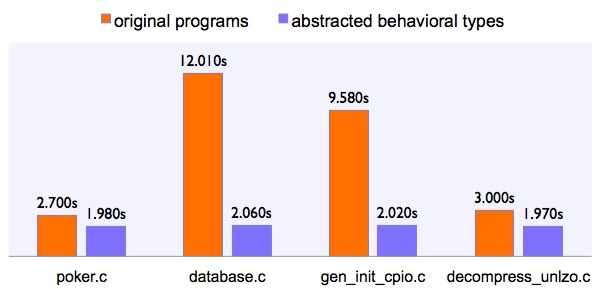
\includegraphics[width=0.5\textwidth]{comp.png} 
\caption{Time spent by a model checker}\label{figcomp} 
\end{figure}

\begin{figure}[!hbp] 
\centering 
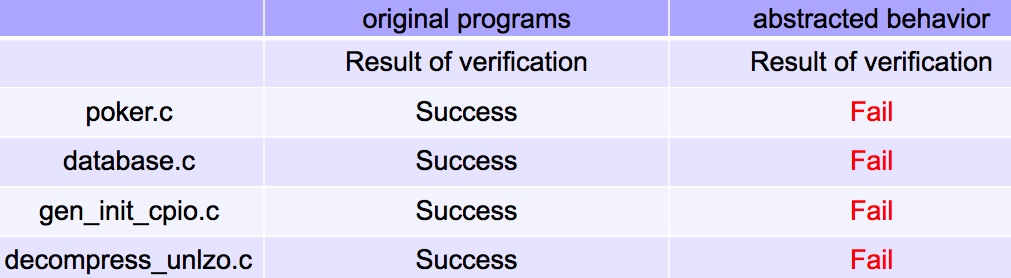
\includegraphics[width=0.5\textwidth]{exp.png} 
\caption{Verification of total memory-leak free}\label{figexp} 
\end{figure}

%% \Begin{table}
%%   \scriptsize
%% \begin{tabular}{|c|c|c|}
%% \hline
%% & \texttt{original programs}  & \texttt{abstracted behavior}  \\
%% \hline
%% & \texttt{result of verification}  & \texttt{result of verification}  \\
%% \hline
%% \texttt{poker.c} & \texttt{Success} & \texttt{Fail} \\
%% \hline
%% \texttt{database.c} & \texttt{Success} & \texttt{Fail} \\
%% \hline
%% \texttt{gen\_init\_cpio.c} &\texttt{Success} & \texttt{Fail} \\
%% \hline
%% \texttt{decompress\_unlzo.c} &\texttt{Success} & \texttt{Fail} \\
%% \hline
%% \end{tabular}
%% \caption{Result of whether the program is total memory-leak free}
%% \label{tb:mcc}
%% \end{table}

\subsection{Accuracy}
From Figure~\ref{figexp}, we observe that verification by applying a
model checker on original programs is Success (totoal memory-leak
free), however, verification on our approach is Fail.

The reason is that our method is not path-sensitive, and it simply
rejects the programs which allocate cells before recursive calls. We
have checked many of source codes from Github and Linux kernel and
found that extending our behavioral type system with dependencies is
useful for our future work.

\section{Related Works}
Many static verification methods have been
proposed~\cite{DBLP:conf/aplas/SuenagaK09,DBLP:conf/pldi/HeineL03,DBLP:conf/sigsoft/XieA05,DBLP:journals/scp/SwamyHMGJ06,DBLP:conf/sas/OrlovichR06,DBLP:conf/issta/SuiYX12}
for memory-leak freedom. These methods guarantee partial memory-leak
freedom and no illegal accesses to deallocated cells, whereas our
behavioral type system guarantees total memory-leak freedom. By using
both their methods and our type system, we can guarantee
safe-memory-deallocation even for nonterminationg programs.

Behavioral types are extensively studied in the context of concurrent
program
verification~\cite{DBLP:conf/esop/HondaVK98,DBLP:journals/tcs/IgarashiK04,DBLP:conf/esop/VieiraCS08,DBLP:journals/lmcs/KobayashiSW06}.
Our type system is largely inspired by one proposed by Kobayashi et
al.~\cite{DBLP:journals/lmcs/KobayashiSW06}, which guarantees that a
concurrent program accesses resources according to specification.

\section{Conclusion}
To verify memory-leak freedom for possibly nonterminating programs, we
proposed a behavioral type system which abstracts the behavior of
programs with allocation and deallocation. We proved the type
soundness and conducted experiments to check feasibility
of our approach.

\section{Future Direction}
The allocation primitives defined in our type system ignore the size
of the allocated block for simplification.  Hence, a memory-leak
program may be checked well-typed by our approach.  Variable-length
cells will be included in our future work.  Another feature should be
considered is path-sensitive, because abstracted behavior types are
not enough to check memory-leak freedom. For accuracy, we are going to
extend our type system with dependencies.


\bibliographystyle{abbrvnat}
\bibliography{tan}

\end{document}


